\section{似然模型}
\zihao{-4}

\label{section:likelihood}

FAIR在本节中提出了一个谈判的基准模型。
作为基准模型,机器至少应能根据输入的项目及其价值模仿人进行谈判。
在此,首先对谈判过程和主体行动进行结构化的分析。
\begin{figure*}[ht!]
\centering
\newcommand{\turnA}{I want the books and the hats, you get the ball}
\newcommand{\turnB}{Give me a book too and we have a deal}
\newcommand{\turnC}{Ok, deal}
\newcommand{\turnD}{\textless choose\textgreater}
\newcommand{\choiceA}{2x\textit{book} 2x\textit{hat}}
\newcommand{\choiceB}{1x\textit{book} 1x\textit{ball}}

\newcommand{\itemvalue}[3]{#2x\textit{#1} & \textit{value}=#3}
\newcommand{\bookA}{\itemvalue{book}{3}{1}}
\newcommand{\hatA}{\itemvalue{hat}{2}{3}}
\newcommand{\ballA}{\itemvalue{ball}{1}{1}}

\newcommand{\bookB}{\itemvalue{book}{3}{2}}
\newcommand{\hatB}{\itemvalue{hat}{2}{1}}
\newcommand{\ballB}{\itemvalue{ball}{1}{2}}

\newcommand{\goals}[3]{
\setlength{\tabcolsep}{0.2em} % for the horizontal padding
\begin{tabular}{ll}
     #1\\#2\\#3
\end{tabular}
}


\tikzstyle{arrow} = [thick,->]
\tikzset{>=latex}

\begin{tikzpicture} 
  \tikzstyle{box} = [rectangle, rounded corners, font=\sffamily\footnotesize, text width=2.45cm, draw=black]
  
  
      \node [box, draw=black, thick, fill = white, minimum width = 6.7cm, minimum height = 8cm]  at (current page.north west) (raw)
    {};
    
    \node[below right] at (raw.north west) (rawlabel) {\underline{\bfseries Crowd Sourced Dialogue
}};
    
  
    \node [box, fill=blue!30, text width      = 2.45cm, below=0.0cm of rawlabel.south west, anchor=north west, xshift=0.2cm]
    (User1Goals)
    {\underline{\bfseries Agent 1 Input}\\
      \goals{\bookA}{\hatA}{\ballA}   
     };
     
    \node [box, right = 0.8cm of User1Goals, fill = blue!30, text width      = 2.45cm]
    (User2Goals)
    {\underline{\bfseries Agent 2 Input}\\
      \goals{\bookB}{\hatB}{\ballB}   
    };
      
    \node [box, below = 0.9cm of User1Goals.south west, anchor=north west, fill = yellow, text width      = 6cm]
    (Dialog)
    {\underline{\bfseries Dialogue}\\
      \textbf{Agent 1:} \turnA\\
      \textbf{Agent 2:} \turnB\\
      \textbf{Agent 1:} \turnC\\
      \textbf{Agent 2:} \turnD\\

    }; 
    
    \node [box, below = 0.8cm of Dialog.south west, anchor=north west, fill = red!30, text width=2.3cm]
    (User1Choice)
    {\underline{\bfseries Agent 1 Output}\\
      \choiceA\\      
    };

    \node [box, right = 1.2cm of User1Choice, fill = red!30, text width=2.3cm]
    (User2Choice)
    {\underline{\bfseries Agent 2 Output}\\
      \choiceB\\      
    };


    \node [box, right = 1cm of raw.north east, ,anchor=north west, draw=black, thick, fill = white, minimum width = 8cm, minimum height = 3.75cm] (perspective1)
    {};
    
    
    \draw [arrow] (User1Goals) -- (Dialog);
    \draw [arrow] (User2Goals) -- (Dialog);
    \draw [arrow] (Dialog) -- (User1Choice);
    \draw [arrow] (Dialog) -- (User2Choice);

    
    
    \node[below right] at (perspective1.north west) (perspective1label) {\underline{\bfseries Perspective: Agent 1}};


    \node [box, below = 0.5cm of perspective1, draw=black, thick, fill = white, minimum width = 8cm, minimum height = 3.75cm] (perspective2)
    {};
    
    \node[below right] at (perspective2.north west) (perspective2label) {\underline{\bfseries Perspective: Agent 2}};


    \node [box, fill = blue!30, text width      = 2.45cm, below=0.0cm of perspective1label.south west, anchor=north west, xshift=0.2cm]
    (perspective1_goals)
    {\underline{\bfseries Input}\\
      \goals{\bookA}{\hatA}{\ballA}   
     };
     
         \node [box, fill = red!30, text width      = 2.45cm, below = 0.2cm of perspective1_goals]
    (perspective1_choice)
    {\underline{\bfseries Output}\\
      \choiceA\\      
     };

    \node [box, right = 1cm of perspective1_goals.north east, anchor=north west, fill = yellow, text width      = 3.5cm]
    (perspective1_dialog)
    {\underline{\bfseries Dialogue}\\
      \textbf{write:} \turnA\ \textbf{read:} \turnB\ 
      \textbf{write:} \turnC\ \textbf{read:} \turnD
    }; 
    
        \node [box, fill = blue!30, text width      = 2.45cm, below=0.0cm of perspective2label.south west, anchor=north west, xshift=0.2cm]
    (perspective2_goals)
    {\underline{\bfseries Input}\\
      \goals{\bookB}{\hatB}{\ballB}   
     };
    
        \node [box, right = 1cm of perspective2_goals.north east, anchor=north west, fill = yellow, text width      = 3.5cm]
    (perspective2_dialog)
    {\underline{\bfseries Dialogue}\\
      \textbf{read:} \turnA\ 
      \textbf{write:} \turnB\ 
      \textbf{read:} \turnC\ 
      \textbf{write:} \turnD
    }; 
    
             \node [box, fill = red!30, text width      = 2.45cm, below = 0.2cm of perspective2_goals]
    (perspective2_choice)
    {\underline{\bfseries Output}\\
      \choiceB\\      
     };
    
    \draw [arrow] (perspective1_goals) -- (perspective1_dialog);
    \draw [arrow] (perspective2_goals) -- (perspective2_dialog);

    \draw [arrow] (perspective1_dialog) -- (perspective1_choice.east);
    \draw [arrow] (perspective2_dialog) -- (perspective2_choice.east);
\end{tikzpicture}
\caption{\label{figure:representation} 谈判过程展示 }
\end{figure*}


\subsection{Date Representation}
\label{subsection:date_representation}

模型将各项目数量、各代理的价值函数作为输入,表示为input goal $\vec{g}$,
其中$\vec{g}$由6个非负整数组成,依次对应各项目的数量和价值;
将代理间的对话作为中间过程,表示为对话dialogue $\vec{x}$,
其中tokens $x_{0..T}$表示对话$\vec{x}$中依次进行的对话;
将代理的输出作为模型输出,表示为output $\vec{o}$,
其中$\vec{o}$由6个非负整数组成,表示三种项目分配给两位代理的数量。

以图\ref{figure:representation}为例,
从每个代理的角度将对话(图\ref{figure:representation}左)分为了两个对话示例(图\ref{figure:representation}右)。

模型的输入为:3本书、2顶帽子、1个球和各代理的价值函数。
其中,对于代理1即\quotes{Agent 1},各项目的单位价值分数分别为:1、3和1,即输入为\quotes{3 1 2 3 1 1};
对于代理2即\quotes{Agent 2},各项目的单位价值分数分别为:2、1和2,即输入为\quotes{3 2 2 1 1 2};
对于每一位代理,因谈判的目的是瓜分资源而不是交易资源,所以输入项目相同且项目总数在5-7之间,项目价值总分均为10。

模型的中间过程根据代理的不同,划分为了两种情况。
其中,对于代理1,首句行为为写\quotes{write},对于代理2,首句行为为读\quotes{read}。

模型的输出为\quotes{2 2 0 1 0 1}。
其中前三位整数\quotes{2 2 0}表示代理1通过谈判认为自己可取得的项目数量,即2本书和2顶帽子;
后三位整数\quotes{1 0 1}表示代理2通过谈判认为自己可取得的项目数量,即1本书和1个球。

值得注意的是,在图\ref{figure:representation}中,因为两个代理输出中各项目选择加起来等于各项目总数,
因此图\ref{figure:representation}中的谈判视为达成,即\quotes{Deal}。
若出现两个代理输出中各项目选择加起来不等于各项目总数,如输出为\quotes{3 2 0 1 0 1},
则表示谈判失败,即\quotes{No Deal}。

\subsection{GRUs RNN}
\label{subsection:grus_rnn}

FAIR在本节中,提出了一个序列-序列网络,以根据代理的输入产生代理的对话,如图\ref{figure:model:supervised}。

模型使用了\citet{  Cho-18,  Cho-28}中提出的循环神经网络,即\quotes{recurrent neural network},
并借鉴了其文章中所提出的\quotes{RNN Encoding-Decoding}机制。
该机制作为此篇论文处理对话自然语言的基础,且文中并未介绍,因此有必要在此就其关键概念进行阐述。
\begin{figure*}[ht!]
    \centering
    \begin{minipage}{0.5\textwidth}
        \centering
        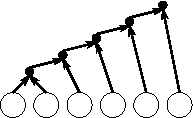
\includegraphics[width=0.5\textwidth]{rnn.pdf}
        \subcaption{\label{figure:rnn} RNN}
    \end{minipage}%
    \begin{minipage}{0.5\textwidth}
        \centering
        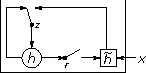
\includegraphics[width=0.5\textwidth]{hidden_unit.pdf}
        \subcaption{\label{figure:gated_unit} Gated Recurrent Unit}
    \end{minipage}%
    \caption{\label{figure:gated_rnn} GRUs RNN}
\end{figure*}

不同于传统的FNN(Feed-forward Neural Networks,前向反馈神经网络),
RNN引入了循环来处理序列数据。典型的序列数据如文本,由一定顺序组成的词构成。
在传统的神经网络模型中,从输入层到隐藏层再到输出层,层与层之间为全连接,但每层之间的节点是无连接的。
这种简单的神经网络对于很多问题无能为力,以翻译模型为例,要预测输出句子即输出词的组合,
需要考虑上文甚至上下文的情景,因为句子中的前后单词并不是独立的。

RNN之所以称为循环神经网络,是因其序列的当前输出与前面的输出有关,如图\ref{figure:rnn}所示。
具体表现形式为,网络会通过激活函数和误差传递对前面的信息进行记忆并应用至当前输出的计算中,
即隐藏层之间的节点不再无连接而是有连接的。
如对于可变长度序列$\vx=(x_1, \dots, x_T)$,对于每一步$t$,隐藏层单元$\vh_{\qt{t}}$的更新公式为:
\begin{equation}
    \label{eq:rnn_hidden_unit_update}
    \vh_{\qt{t}} = f\left( \vh_{\qt{t-1}}, x_t \right)
\end{equation}

其中$f$为非线性激活函数。通过将词的预测转化为词概率的计算问题,
RNN可以通过学习预测出下一个输出的所有词的概率,通过选择概率最大的词完成预测。
如共有$K$个词,则第$t$个词$x_{t,j}$的计算公式为:
\begin{equation}
    \label{eq:rnn_word_prediction}
    p(x_{t,j} = 1 \mid x_{t-1}, \dots, x_1) = \frac{\exp \left(
        \vw_j \vh_{\qt{t}}\right) } {\sum_{j'=1}^{K} \exp \left( \vw_{j'}
        \vh_{\qt{t}}\right) }
\end{equation}

其中$j$表示所有可能的词,$j=1,\dots,K$,
$\vw_j$是词权重矩阵$\mW$的列。
通过组合词的概率,从而完成词序列$\vx$的预测。
\begin{equation}
    % \label{eq:distribution}
    p(\vx) = \prod_{t=1}^T p(x_t \mid x_{t-1}, \dots, x_1)
\end{equation}

因为这一特性,RNN及其改进型被广泛应用于机器翻译模型中。
\citet{  Cho-28}在此基础上提出了适用于统计机器翻译的词嵌入方法与Encoder-Decoder机制,
如图\ref{figure:rnn_encdec}。
\begin{figure*}[ht!]
    \centering
    \begin{minipage}{0.4\textwidth}
        \centering
        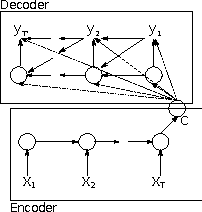
\includegraphics[width=0.4\textwidth]{unit_encdec.pdf}
        \subcaption{\label{figure:unit_encdec} Units Encode-Decode}
    \end{minipage}%
    \begin{minipage}{0.6\textwidth}
        \centering
        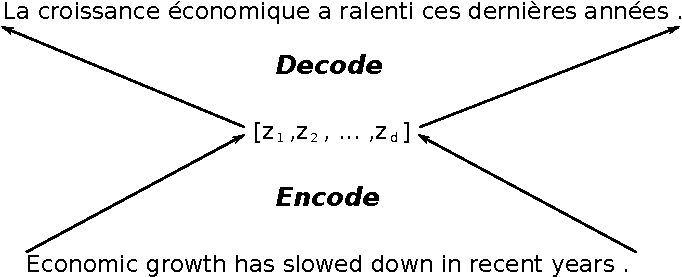
\includegraphics[width=0.6\textwidth]{seq_encdec.pdf}
        \subcaption{\label{figure:seq_encdec} Sequence Encode-Decode}
    \end{minipage}%
    \caption{\label{figure:rnn_encdec} RNN Encode-Decode}
\end{figure*}
在现实情况下,序列数据的输入一般都是可变长度的。
图\ref{figure:unit_encdec}展示了将可变长度的序列数据$\vx=(x_1, \dots, x_T)$作为输入嵌入至矩阵$c$,
然后再以$c$和目标序列数据$\vy=(y_1, \dots, y_{T-1'})$作为输入,生成$\vy=(y_1, \dots, y_{T'})$。

值得注意的是,这里的$T$和$T'$可能是不同的。

此时,隐藏层单元$\vh_{\qt{t}}$的更新公式为:
\begin{equation}
    % \label{eq:decode_hidden_unit_update}
    \vh_{\qt{t}} = f\left( \vh_{\qt{t-1}}, y_{t-1}, \vc \right)
\end{equation}

同样的,目标词$y_t$的计算公式为:
\begin{equation}
    P(y_t | y_{t-1}, y_{t-2}, \ldots, y_1, \vc) = g\left(\vh_{\qt{t}}, y_{t-1}, \vc \right)
\end{equation}


理论上,RNN能对任何长度的序列数据进行处理,但是由于梯度消失和梯度爆炸问题,
实际运用中多使用改进型RNN,如图\ref{figure:gated_unit}所示,便是Gated Recurrent Unit(GRU)。
结合GRU的改进型Gated Recurrent Units RNN即为此篇论文所使用GRUs。

以图\ref{figure:gated_unit}和图\ref{figure:seq_encdec}为例。
以$x=(\vx_1, \vx_2, \cdots, \vx_T)$表示输入的序列数据,其中$\vx_t \in\RR^d$。
GRUs由四个权重矩阵组成,分别为$\mW^l$、$\mW^r$、 $\mG^l$和$\mG^r$。
对于任意一步$t \in \left[ 1, T-1\right]$,第$j$个隐藏层单元$h^{(t)}_j$计算为:
\begin{equation}
    % \label{eq:grconv_main}
    h^{(t)}_j = \omega_c \tilde{h}^{(t)}_j + \omega_l h^{(t-1)}_{j-1} + \omega_r h^{(t-1)}_j
\end{equation}

其中$\omega_c$、$\omega_l$和$\omega_r$值的和为$1$。隐藏层单元初始化为:
\begin{equation}
    h^{(0)}_j = \mU \vx_j
\end{equation}

其中$\mU$表示输入数据的隐藏层映射矩阵。

新的激活函数$\tilde{h}^{(t)}_j$计算为:
\begin{equation}
    \tilde{h}^{(t)}_j = \phi\left( \mW^l h^{(t)}_{j-1} + \mW^r h^{(t)}_{j}
    \right),
\end{equation}

其中$\phi$为非线性激活函数。

聚集系数$\omega$计算为:
\begin{equation}
    \left[ 
        \begin{array}{c}
            \omega_c \\
            \omega_l \\
            \omega_r
        \end{array}
    \right] = \frac{1}{Z}
    \exp\left( \mG^l h^{(t)}_{j-1} + \mG^r h^{(t)}_{j}
    \right)
\end{equation}

其中$\mG^l, \mG^r \in \RR^{3 \times d}$且
\begin{equation}
    Z = \sum_{k=1}^3 \left[\exp\left( \mG^l h^{(t)}_{j-1} + \mG^r h^{(t)}_{j} \right)\right]_k.
\end{equation}

由此完成了基于GRUs RNN的词嵌入与Encode-Decode机制。
\citet{  Cho-18,  Cho-28}利用该机制实现了一个英译法的统计机器翻译模型。

\subsection{Supervied Learning}
\label{subsection:supervised_learning}

如\ref{subsection:grus_rnn}中所提,FAIR在本小节中,提出了一个序列-序列网络,以根据代理的输入产生代理的输出。
其中,
该序列-序列网络,或称为端到端网络,是在\citet{  Cho-18,  Cho-28}所提的GRUs RNN Encode-Decode基础上的应用与改进\wordnote{
    与\citet{  Cho-18,  Cho-28}相同的是,此篇论文的对话输入和输出也均是文本序列数据;
    不同在于,此篇论文的输入中包含了项目数量和价值,并希望最终输出取得最大的价值分数,而不仅是流畅地进行谈判对话。
};
代理的输入包含初始项目数量、价值和对话;
代理的输出包含对话和选择。

因此此篇论文所提的端到端网络模型使用了四个RNN:
$\text{GRU}_w$,$\text{GRU}_g$,$\text{GRU}_{\overrightarrow{o}}$和$\text{GRU}_{\overleftarrow{o}}$。

\def\layersep{1.0cm}
%\newcommand{\counts}[2]{\textit{#2x}\textbf{#1}}
\newcommand{\counts}[2]{\textbf{#1} \textit{count}=#2}
\newcommand{\values}[2]{\textbf{#1} \textit{value}=#2}


\def\goals{}%\counts{book}{3}, \values{book}{2}, \counts{hat}{2}, \values{hat}{1}, \counts{ball}{1}, \values{ball}{2}, \values{ball}{2}}

    \tikzstyle{every pin edge}=[<-,shorten <=1pt]
    \tikzstyle{neuron}=[circle,fill=black!25,minimum size=17pt,inner sep=0pt]
    \tikzstyle{input neuron}=[neuron,draw=black!50, fill=white]
    \tikzstyle{output neuron}=[neuron, fill=red!50]
    \tikzstyle{hidden neuron}=[neuron, fill=blue!50]
    \tikzstyle{annot} = [text width=4em, text centered]
  \tikzstyle{box} = [rectangle, rounded corners, font=\sffamily\footnotesize, text width=2.3cm, draw=black]

\newcommand{\network}[0]{
\scalebox{0.7}{
\begin{tikzpicture}[shorten >=1pt,->,draw=black!50, node distance=\layersep]
\tikzset{>=latex}

  
  
      \node [box, draw=black, thick, fill = white%, minimum width = 2.7cm, minimum height = 1cm
      ] at (2,0.2) (enc) {Input Encoder};

      \node [box, draw=black, thick, fill = white%, minimum width = 2.7cm, minimum height = 1cm
      , right = 1cm of enc]  (dec) {Output Decoder};

   

    \foreach[count=\y,evaluate=\y as \prevx using int(\y-2)] \name in \words {
        \node[input neuron] (H-\y) at (\prevx, -2) {};
        \node[anchor=base] (O-\y) at (\prevx, -3) {\name};
    }

    \foreach[count=\y,evaluate=\y as \prevx using int(\y-1)] \w in \written {
        \ifthenelse{\y>1}{\path (O-\prevx) edge (H-\y);}{}
        \ifthenelse{\y>1}{\path (H-\prevx) edge (H-\y);}{}
        \ifthenelse{\y>0 \AND \w=1}{\path (H-\y) edge (O-\y);}{}
        

        \path (enc) edge (H-\y);
        \path (H-\y) edge (dec);
    }


%[evaluate=\x as \evalx using int(\x+1)]
\end{tikzpicture}
}
}



\begin{figure*}[t!]
    \def\words{\you,\vphantom{.}\space\space Take, one, hat, \them, I, need, two, \you, deal, \dots}

    \centering
    \begin{subfigure}[t]{0.5\textwidth}
        \def\written{1, 1, 1, 1, 1, 1, 1, 1, 1, 1, 1}
        \centering
        \network
        \caption{\label{figure:model:supervised} Supervised Training}
    \end{subfigure}%
    ~ 
    \begin{subfigure}[t]{0.5\textwidth}
        \def\written{0, 1, 1, 1, 1, 0, 0, 0, 0, 1, 1}
        \centering
        \network
        \caption{\label{figure:model:reinforcement} Decoding, and Reinforcement Learning}
    \end{subfigure}
    \caption{\label{figure:model} 端到端神经网络}
\end{figure*}
代理的输入$\vec{g}$通过$\text{GRU}_g$进行Encode,对应的隐藏层单元为$h^g$。
模型基于$h^g$和$x_{t-1}$对$x_t$进行依次预测。
对于每一步$t$, $\text{GRU}_w$都将
上一隐藏层单元$h_{t-1}$、上一词$x_{t-1}$\wordnote{
    通过矩阵$E$进行词嵌入。
}和$h^g$
作为神经网络的输入,以更新当前的隐藏层单元$h_t$。
\begin{equation}
h_t = \text{GRU}_w(h_{t-1}, [Ex_{t-1}, h^g])
\end{equation}

因此,目标词$x_t$的计算关系为:
\begin{equation}
p_\theta (x_t | x_{0.. t-1}, \vec{g}) \propto \exp(E^T h_t)
\end{equation}

值得注意的是,此时的模型会同时预测两位代理的对话词,并且模型依然是前馈的。

在对话的最后,代理会输出选择,以$\vec{o}$表示。
在这里,模型对两位代理的选择通过相互独立的分类器独立预测\wordnote{
    这也是为什么要在\ref{subsection:date_representation}中需要对代理分开进行建立输入、中间过程和输出的原因。
}。
分类器通过对话共享双向$\text{GRU}_o$模型和Attention机制\citep{BaarslagFujita-17},
在对话和$\vec{g}$的基础上进行词预测。
\begin{align}
h^{\overrightarrow{o}}_t &= \text{GRU}_{\overrightarrow{o}}(h^{\overrightarrow{o}}_{t-1}, [Ex_{t}, h_t])\\
h^{\overleftarrow{o}}_t &= \text{GRU}_{\overleftarrow{o}}(h^{\overleftarrow{o}}_{t+1}, [Ex_{t}, h_t])\\
h^o_t&=[h^{\overleftarrow{o}}_t, h^{\overrightarrow{o}}_t]\\
h^a_t&=W[\tanh(W'h^o_t)]\\
\alpha_t &= \frac {\exp(w \cdot h^a_t)}{\sum_{t'} \exp(w\cdot h^a_{t'})}
\end{align}
\begin{equation}
h^s = \tanh(W^s[h^g, \sum_t \alpha_t h_t])
\end{equation}

最终的选择则在对话、$\vec{g}$和$h^s$的基础上预测,计算关系为:
\begin{equation}
p_\theta(o_i | x_{0..t}, \vec{g}) \propto \exp(W^{o_i} h^s)
\end{equation}

模型通过降低对话预测损失和选择预测损失来实现较好的预测效果。
两个误差间的权重通过$\alpha$来调节。
\begin{equation}
\label{eq:supervised}
L(\theta) = -\underbrace{\sum_{\vec{x},\vec{g}} \sum_{t} \log p_\theta(x_t | x_{0.. t-1}, \vec{g})}_{\text{Token prediction loss}} - \alpha \underbrace{\sum_{\vec{x},\vec{g},\vec{o}} \sum_{j} \log p_\theta(o_j | x_{0.. T}, \vec{g})}_{\text{Output choice prediction loss}}
\end{equation}

不同于\citet{VinyalsLe-19}的神经网络对话模型,FAIR的方法考虑和共享了读取和写入词的所有参数。

\subsection{Decoding}
\label{subsection:decoding}

在Decoding的过程中,模型必须要根据对话历史$x_{0..t-1}$和输入项目数量与价值$\vec{g}$产生$x_{0..T}$。
如同\ref{subsection:grus_rnn}中的Decode过程,也是通过选取最大概率词的方式进行预测。计算关系为:
\begin{equation}
 x_t \sim p_\theta(x_t | x_{0..t-1}, \vec{g})
\end{equation}

整个对话过程以任一一方代理写出结束标志词\wordnote{
    \emph{end-of-dialogue},即结束标志词,如\quotes{Deal}、\quotes{OK}和\quotes{Okey}等。
}时结束。这时模型预测出选择$\vec{o}$,具体为从满足约束条件的可行输出选择集$O$中选择概率最高的那个。
\begin{equation}
\label{equation:output}
\vec{o}^{*} = \argmax_{\vec{o}\in O} \prod_{i} p_\theta(o_i | x_{0.. T}, \vec{g})
\end{equation}

值得注意的是,此篇论文在这里使用了\quotes{feasible set}一词。
个人通过实验推测其原因为:若不建立可行输出选择集,直接选取概率最高的输出选择,可能会出现该选择不满足约束条件,
即可能项目数量直接高于初始项目数量的情况。此时已不属于谈判失败,而属于代理非智能。
因此,FAIR在这里建立了可行输出集。
同时FAIR在初始项目数量时,设置了总数在5-7间的规定,有效降低了枚举可行输出选择的时间复杂度。
因此FAIR在设立这一规定时就考虑了这一因素,这个技巧非常巧妙,值得借鉴。